\documentclass[]{article}
\usepackage{lmodern}
\usepackage{amssymb,amsmath}
\usepackage{ifxetex,ifluatex}
\usepackage{fixltx2e} % provides \textsubscript
\ifnum 0\ifxetex 1\fi\ifluatex 1\fi=0 % if pdftex
  \usepackage[T1]{fontenc}
  \usepackage[utf8]{inputenc}
\else % if luatex or xelatex
  \ifxetex
    \usepackage{mathspec}
  \else
    \usepackage{fontspec}
  \fi
  \defaultfontfeatures{Ligatures=TeX,Scale=MatchLowercase}
\fi
% use upquote if available, for straight quotes in verbatim environments
\IfFileExists{upquote.sty}{\usepackage{upquote}}{}
% use microtype if available
\IfFileExists{microtype.sty}{%
\usepackage{microtype}
\UseMicrotypeSet[protrusion]{basicmath} % disable protrusion for tt fonts
}{}
\usepackage[margin=1in]{geometry}
\usepackage{hyperref}
\hypersetup{unicode=true,
            pdfborder={0 0 0},
            breaklinks=true}
\urlstyle{same}  % don't use monospace font for urls
\usepackage{graphicx,grffile}
\makeatletter
\def\maxwidth{\ifdim\Gin@nat@width>\linewidth\linewidth\else\Gin@nat@width\fi}
\def\maxheight{\ifdim\Gin@nat@height>\textheight\textheight\else\Gin@nat@height\fi}
\makeatother
% Scale images if necessary, so that they will not overflow the page
% margins by default, and it is still possible to overwrite the defaults
% using explicit options in \includegraphics[width, height, ...]{}
\setkeys{Gin}{width=\maxwidth,height=\maxheight,keepaspectratio}
\IfFileExists{parskip.sty}{%
\usepackage{parskip}
}{% else
\setlength{\parindent}{0pt}
\setlength{\parskip}{6pt plus 2pt minus 1pt}
}
\setlength{\emergencystretch}{3em}  % prevent overfull lines
\providecommand{\tightlist}{%
  \setlength{\itemsep}{0pt}\setlength{\parskip}{0pt}}
\setcounter{secnumdepth}{0}
% Redefines (sub)paragraphs to behave more like sections
\ifx\paragraph\undefined\else
\let\oldparagraph\paragraph
\renewcommand{\paragraph}[1]{\oldparagraph{#1}\mbox{}}
\fi
\ifx\subparagraph\undefined\else
\let\oldsubparagraph\subparagraph
\renewcommand{\subparagraph}[1]{\oldsubparagraph{#1}\mbox{}}
\fi

%%% Use protect on footnotes to avoid problems with footnotes in titles
\let\rmarkdownfootnote\footnote%
\def\footnote{\protect\rmarkdownfootnote}

%%% Change title format to be more compact
\usepackage{titling}

% Create subtitle command for use in maketitle
\providecommand{\subtitle}[1]{
  \posttitle{
    \begin{center}\large#1\end{center}
    }
}

\setlength{\droptitle}{-2em}

  \title{}
    \pretitle{\vspace{\droptitle}}
  \posttitle{}
    \author{}
    \preauthor{}\postauthor{}
    \date{}
    \predate{}\postdate{}
  
% Allowing for landscape pages
\usepackage{lscape}
\usepackage{booktabs}
\usepackage{multirow}
\usepackage{float}
\usepackage{placeins}
\newcommand{\blandscape}{\begin{landscape}}
\newcommand{\elandscape}{\end{landscape}}

% Left justification of the text: see https://www.sharelatex.com/learn/Text_alignment
% \usepackage[document]{ragged2e} % already in the latex template
\newcommand{\bleft}{\begin{flushleft}}
\newcommand{\eleft}{\end{flushleft}}

\begin{document}

\listoffigures

\newpage

(ref:foo) Correlation between EPSPS-inhibitor resistant \emph{Amaranthus
palmeri} individuals with glyphosate and molecular (\emph{EPSPS} gene
amplification) assays. Each dot represent an \emph{A. palmeri} biotype
from southwestern Nebraska

\begin{figure}[h]

{\centering 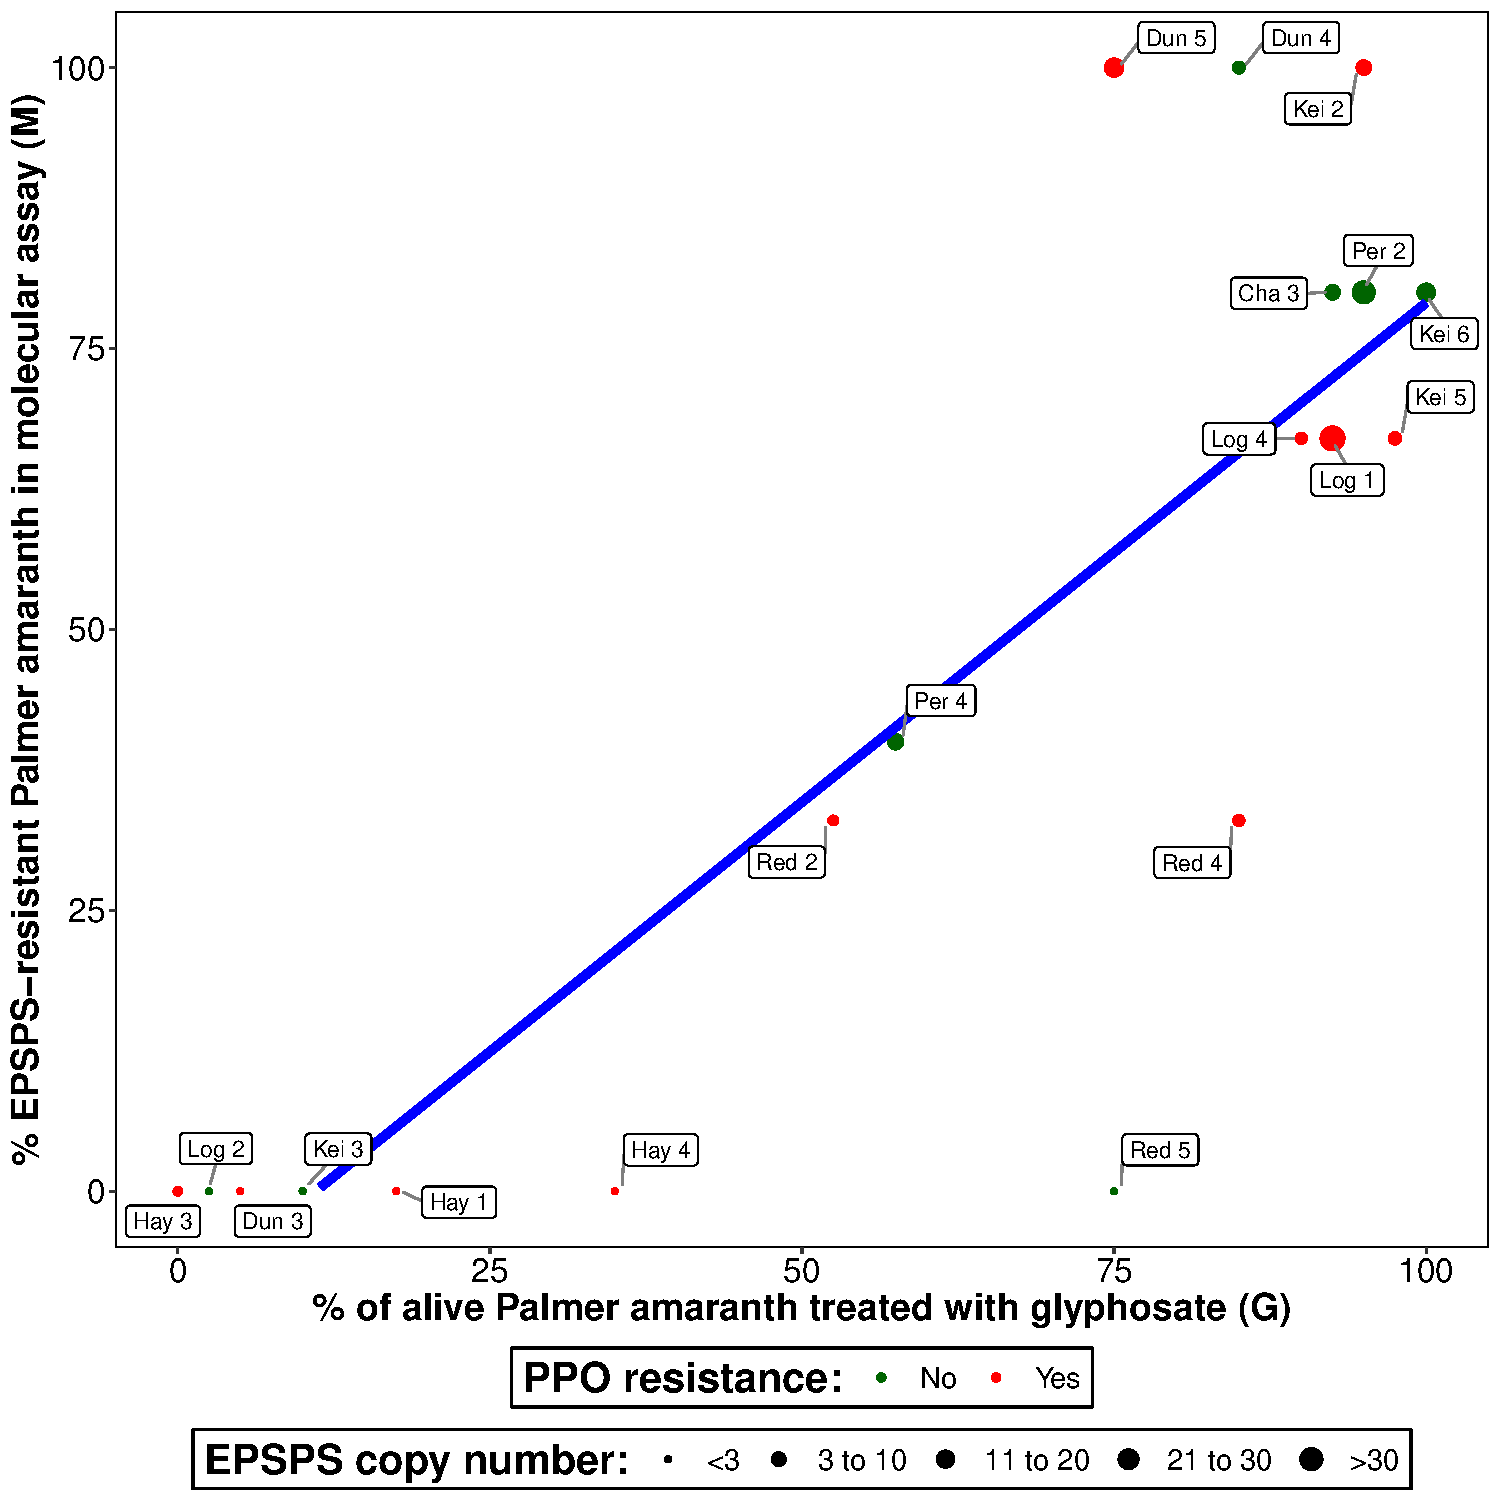
\includegraphics[width=1\linewidth]{Figure 1} 

}

\caption{(ref:foo)}\label{fig:unnamed-chunk-1}
\end{figure}

\newpage

\blandscape

\begin{figure}[h]

{\centering \includegraphics[width=1\linewidth]{Figure 2} 

}

\caption{Correlation between PPO-inhibitor resistant A. palmeri individuals represents fomesafen (A) or lactofen (B) and molecular (EPSPS gene amplification) assays. Each dot represent an A. palmeri biotype from southwestern Nebraska.}\label{fig:unnamed-chunk-2}
\end{figure}

\newpage

\begin{figure}[h]

{\centering \includegraphics[width=1\linewidth]{Figure 3} 

}

\caption{Presence of EPSPS- and/or PPO-inhibitor resistance in 51 Amaranthus palmeri biotypes from southwestern Nebraska}\label{fig:unnamed-chunk-3}
\end{figure}
\elandscape

\begin{figure}[h]

{\centering 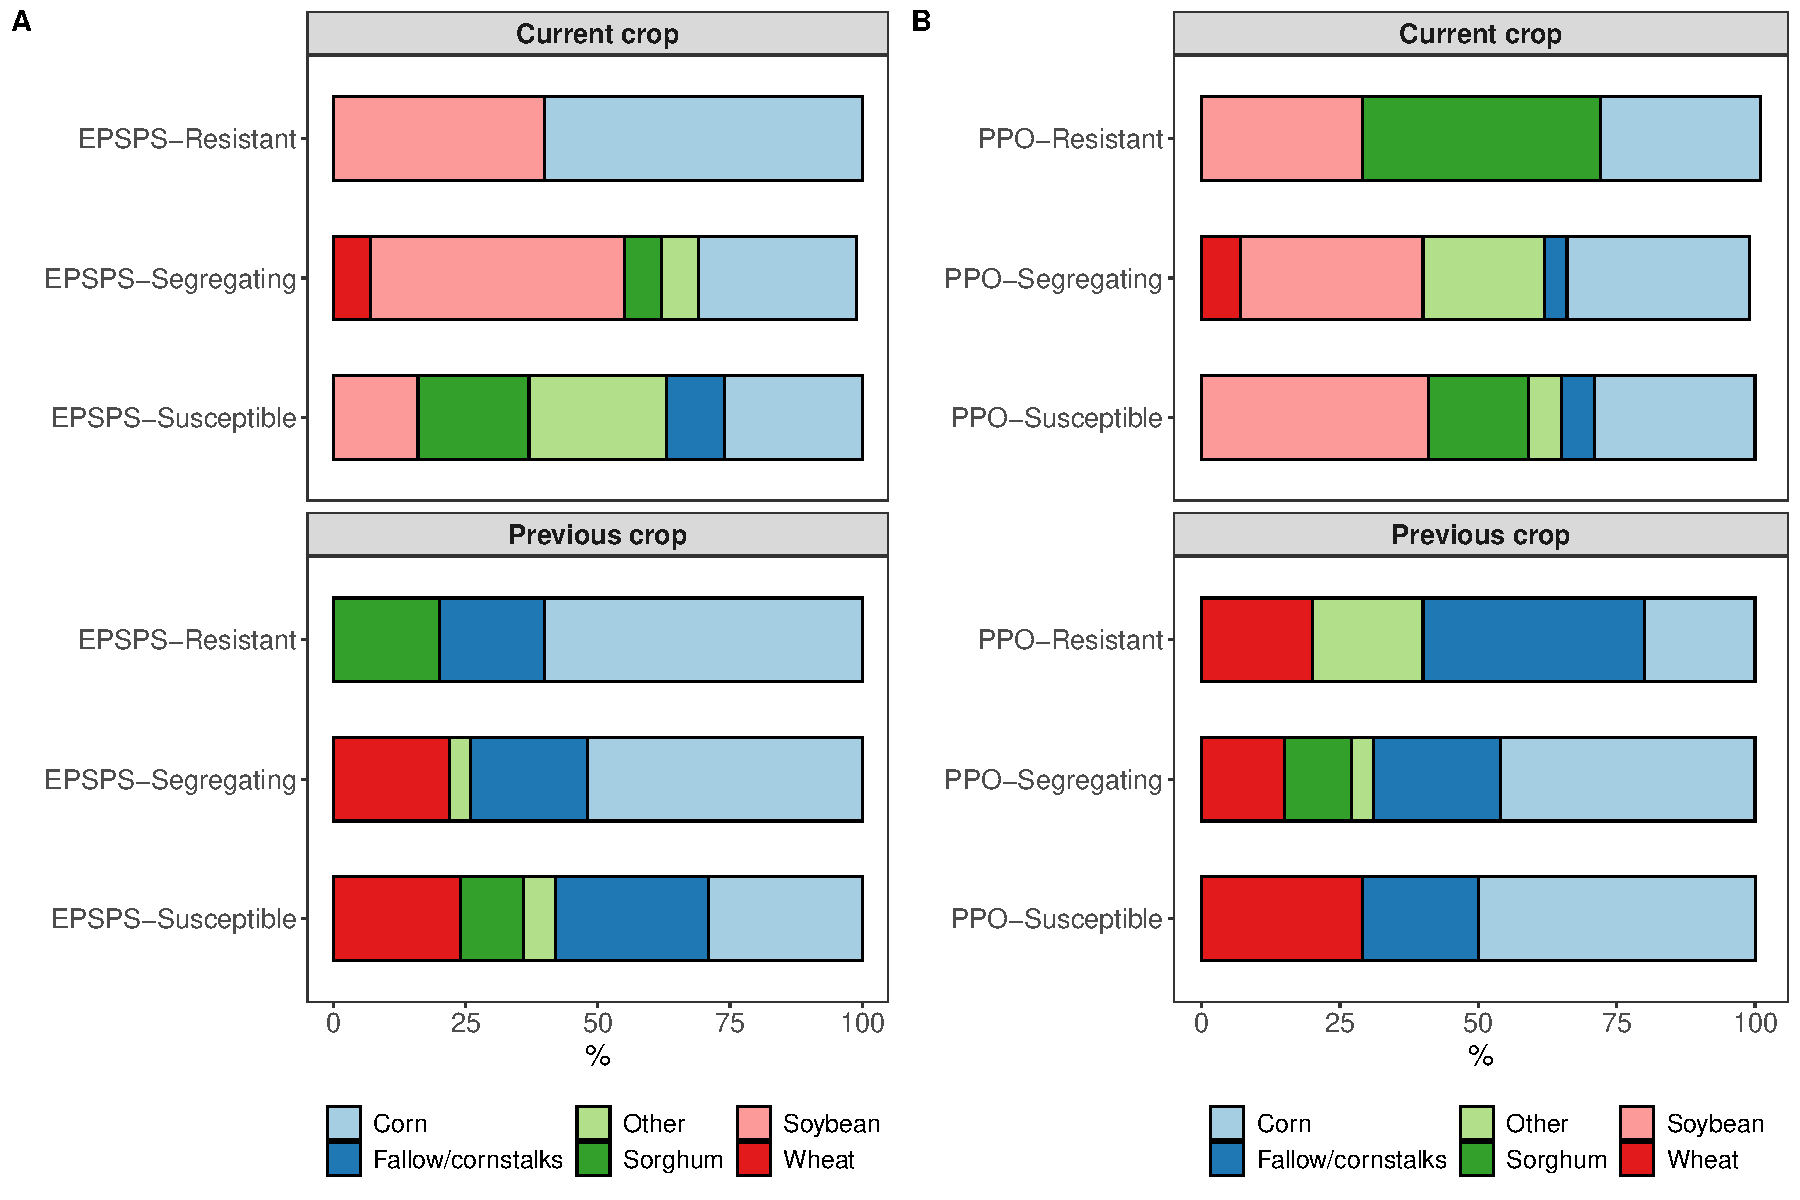
\includegraphics[width=1\linewidth]{Figure 4} 

}

\caption{Random forest analysis of likelihood of EPSPS-inhibitor resistance in Amaranthus palmeri biotypes in response to mechanism of resistance, agronomic practices, and geographic location and weed demographics in southwestern Nebraska. Variables are ordered by importance measured using the Gini coefficient.}\label{fig:unnamed-chunk-4}
\end{figure}

\newpage

\blandscape

\begin{figure}[h]

{\centering \includegraphics[width=1\linewidth]{Figure 5} 

}

\caption{Percentage of diversty in current and previous crop where the EPSPS-(A) and PPO-(B) resistant Amaranthus palmeri biotypes was found in southwestern Nebraska. Biotypes are grouped into EPSPS-Resistant, EPSPS-Segregating and EPSPS-Suceptible representing A. palmeri with all resistant, partially resistant, and no resistant individuals, respectively.}\label{fig:unnamed-chunk-5}
\end{figure}

\elandscape


\end{document}
